
\documentclass[10pt]{article} % Default font size

\usepackage[T1]{fontenc}
\usepackage[polish]{babel}
\usepackage[utf8]{inputenc}
\usepackage{lmodern}
\selectlanguage{polish}
\usepackage{hyperref}
\usepackage{amsmath}
\usepackage{gensymb}
\usepackage{subcaption}
\usepackage{graphicx}
\usepackage{listings}



\begin{document}

\title{%
  Wykorzystanie algorytmu Hougha do detekcji obramowań tabel na dokumentach \\[0.6\baselineskip]
  \large Projekt z przedmiotu CPOO}
\author{Michał Krawczak}

\maketitle

\tableofcontents

\newpage

\section{Temat projektu}

W ramach projektu z przedmiotu CPOO zdecydowałem pochylić się nad problemem, na który natrafiłem podczas prac nad jednym z projektów, które realizowałem w pracy zawodowej, tj. problemem wykorzystania algorytmu Hougha do detekcji linii w dokumentach finansowych. 

\subsection{Zakres projektu}

W ramach niniejszego projektu zaimplementowałem algorytm Hougha w języku Java, a następnie przetestowałem go na obrazach kilku dokumentów, zarówno oryginalnych, jak i celowo zaszumionych. Ponadto, na tych samych obrazach, uruchomiłem gotowy moduł wykonujący algorytm Hougha, wchodzący w skład popularnego pakietu \texttt{imagemagick} \cite{imagemagick}. Następnie dokonałem porównania wyników działania obu tych podejść. 

\section{Algorytm Hougha}

Algorytm Hougha, opisany pierwotnie w \cite{hough}, stał się jednym z podstawowych algorytmów komputerowego przetwarzania obrazów. Najczęstszym zastosowaniem tego algorytmu jest detekcja prostych, jednak można go łatwo zaadaptować do wykrywania dowolnych kształtów, które dają się opisać za pomocą analitycznego wzoru\cite{duda}. Podstawowym pojęciem leżącym u podstaw tej techniki jest transformacja Hougha.

\subsection{Transformacja Hougha}
Transformacja Hougha przekształca przestrzeń kartezjańską w przestrzeń Hougha. Przestrzeń Hougha to dwuwymiarowa przestrzeń, w której każda prosta\footnote{Od tego miejsca zakładam, że wykrywaną figurą jest prosta.} z obrazu oryginalnego jest reprezentowana przez pojedynczy punkt. 

Osie, na których rozpięta jest przestrzeń Hougha, reprezentują następujące skalary:
\begin{itemize}
\item $r$ --- reprezentuje długość najkrótszego odcinka łączącego prostą ze środkiem układu współrzędnych $(0, 0)$ oryginalnego obrazu.
\item $\theta$ --- reprezentuje kąt między ww. odcinkiem, a osią OX oryginalnego obrazu.
\end{itemize}
 
Ponadto, każdy punkt w przestrzeni Hougha ma przypisaną wartość całkowitoliczbową $n$, która oznacza liczbę punktów w obrazie pierwotnym, które spełniają równanie prostej.

\subsection{Pseudokod algorytmu}\label{pseudokod}

Algorytm można zrealizować za pomocą następujących kroków:
\begin{enumerate}
\item Parametry wejściowe: 
 \begin{itemize}
   \item $\delta_\theta$ --- rozmiar kroku $\theta$
   \item $t$ --- próg binaryzacji (tj. graniczna jasność poniżej której piksele mają być uznane za czarne). 
   \item $p$ --- próg filtrowania wyników (tj. minimalna liczba punktów na prostej, aby była ona godna zwrócenia użytkownikowi).
 \end{itemize}
\item Weź obraz wejściowy $I$ o wymiarach $n\times m$.
\item Utwórz tablicę $H$ liczb całkowitych o wymiarach $\theta_s \times d$, gdzie $\theta_s = \dfrac{2\pi}{\delta_\theta}$, $d=\sqrt{n^2+m^2}$ i wypełnij ją zerami.
\item Dla każdego piksela $I_{n,m}$ w obrazie wejściowym $I$:
  \begin{enumerate}
    \item Dla każdej wartości $\theta$ od $0$ do $\pi$ z krokiem co $\delta_\theta$:
  		\begin{enumerate}
    		\item Oblicz $r = \lfloor x \cdot \cos \theta + y \cdot \sin \theta \rfloor$
    		\item Jeśli jasność piksela $I_{n,m}$ jest poniżej progu $t$, to zwiększ wartość $H_{\theta, r}$ o $1$
  		\end{enumerate}
  \end{enumerate}
\item Wybierz te elementy tablicy $H$, których wartość jest większa niż $p$. Zwróć je użytkownikowi.
\end{enumerate}

Wynik może zostać zwrócony w postaci listy prostych, gdzie każda jest opisana przez parę parametrów $(\theta, r)$. Wygodniej jest jednak, jeżeli wynik ma postać graficzną, np. wykryte linie zostają narysowane i nałożone na obraz wejściowy. W takiej postaci zostaną zaprezentowane wyniki w kolejnych rozdziałach.

\section{Implementacja}

Kod programu znajduje się w repozytorium pod adresem: \\
\href{https://github.com/ciekawylogin/hough}{https://github.com/ciekawylogin/hough}

Właściwy kod programu został umieszczony w pliku \texttt{HoughLineDetector.java}. Realizuje on niemal dokładnie algorytm opisany w \ref{pseudokod}. Jedynym drobnym usprawnieniem było wprowadzenie do kroku $5.$ dodatkowego warunku: linie są zwracane tylko wtedy, gdy są lepsze (tj. mają więcej punktów), niż ich 4 bezpośredni sąsiedzi w przestrzeni Hougha. Warunek ten sprawdzany jest w liniach 207--211. Nie wpływa on znacząco na poprawność, a jedynie ogranicza zbiór wynikowy. W oryginalnej postaci algorytm często zwraca grupy bardzo podobnych do siebie linii -- np. obróconych o $1\degree$ albo przesuniętych o 1 piksel. Wprowadzenie tego dodatkowego sprawdzenia powoduje, że zwrócona zostaje tylko jedna (potencjalnie najtrafniejsza) linia z takiej grupy, przez co wynikowy obraz jest czytelniejszy.

\section{Testowanie}

W celu przetestowania powyższego programu i porównania go z narzędziem wchodzącym w skład programu \texttt{imagemagick}, oba programy zostały uruchomione na 5 obrazach testowych.

Własna implementacja była uruchamiana z następującymi parametrami: próg binaryzacji $r=80$, próg algorytmu Hougha $p=400$, rozmiar kroku kątowego $\delta_\theta = \frac{2\pi}{360}$ (tj. 360 kroków).

\texttt{Imagemagick} był wywoływany w następujący sposób:

\begin{lstlisting}
convert <obraz_wejsciowy>.jpg -colorspace gray \
  +dither -colors 2 -normalize -negate -hough-lines \
  100x100+250 -transparent white temp.png 
composite temp.png <obraz_wejsciowy> <obraz_wynikowy>.jpg
rm temp.png
\end{lstlisting}

Powyższa komenda wykonuje binaryzację (z użyciem progowania Otsu), następnie wykonuje algorytm Hougha i zapisuje uzyskane linie do pliku \texttt{temp.png}. Następnie linie są nakładane na oryginalny obraz i tworzony jest obraz wynikowy.

\begin{figure}
  \begin{subfigure}{\linewidth}
  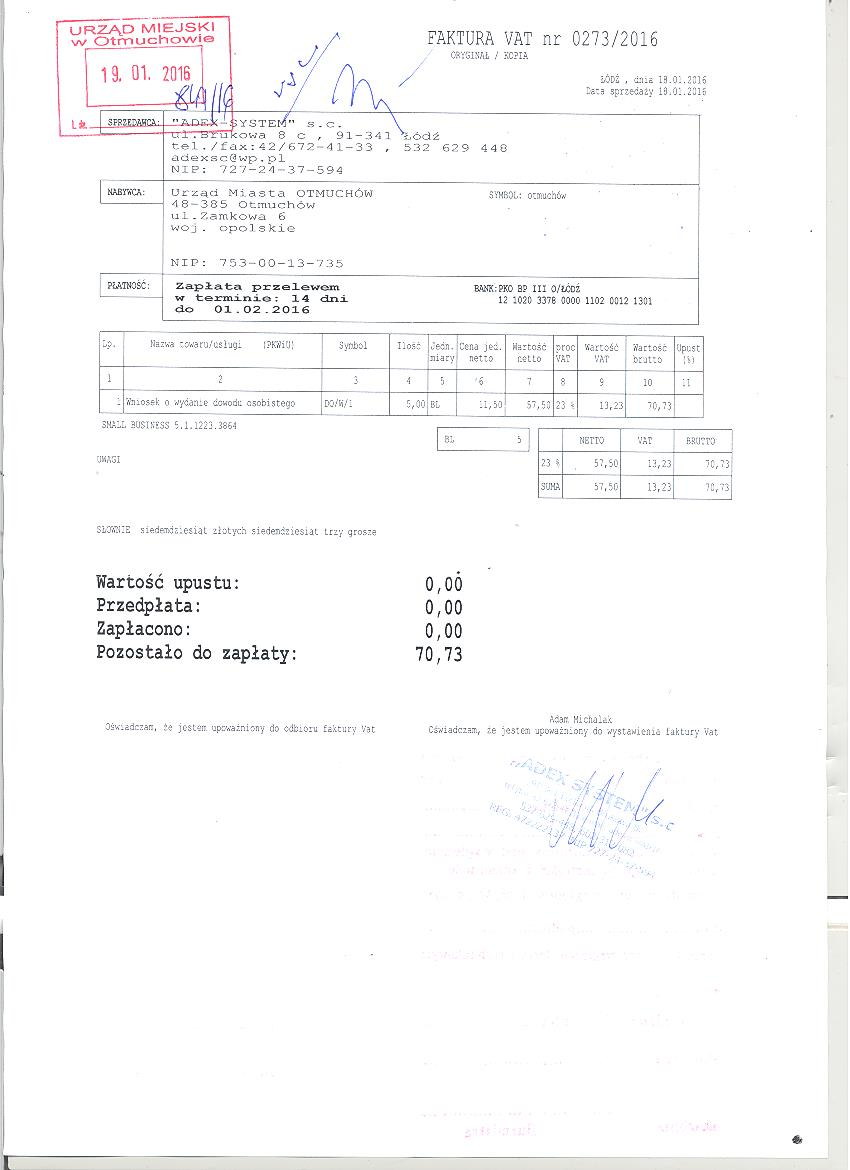
\includegraphics[width=.33\linewidth]{testing/ADEX.jpg}\hfill
  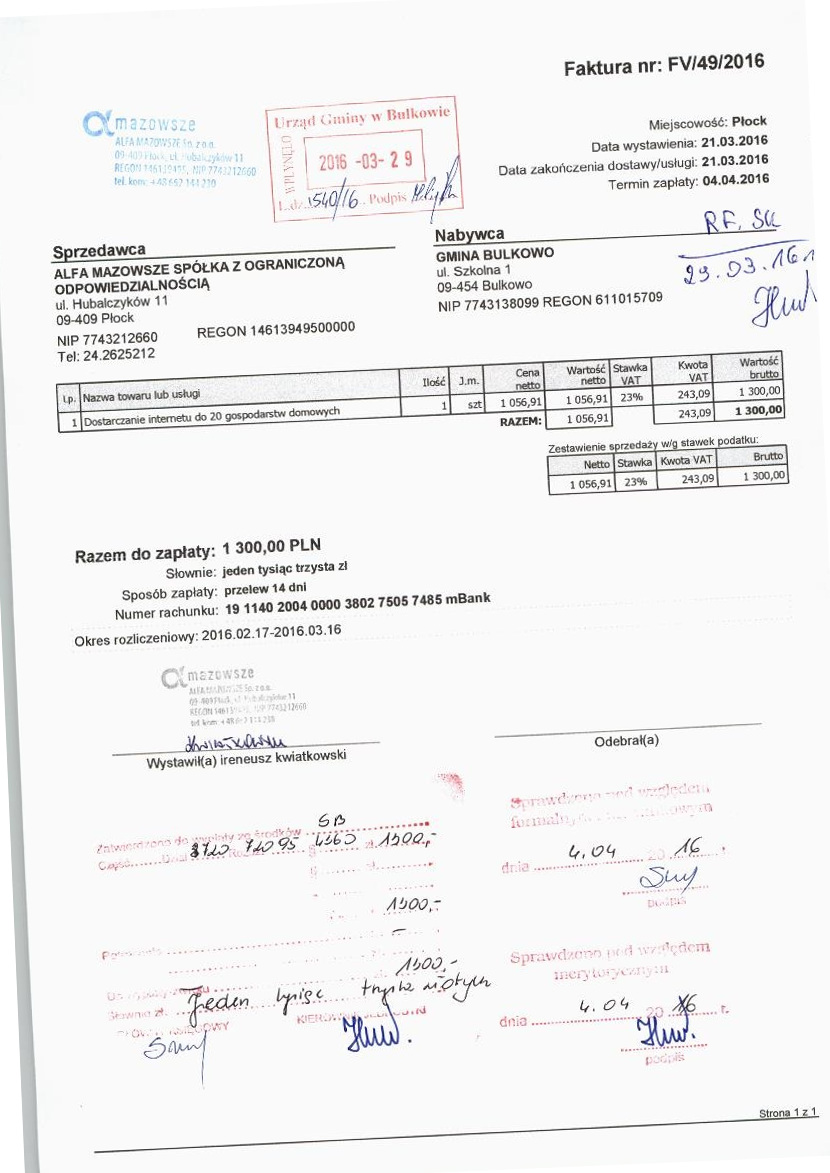
\includegraphics[width=.33\linewidth]{testing/ALFA.jpg}\hfill
  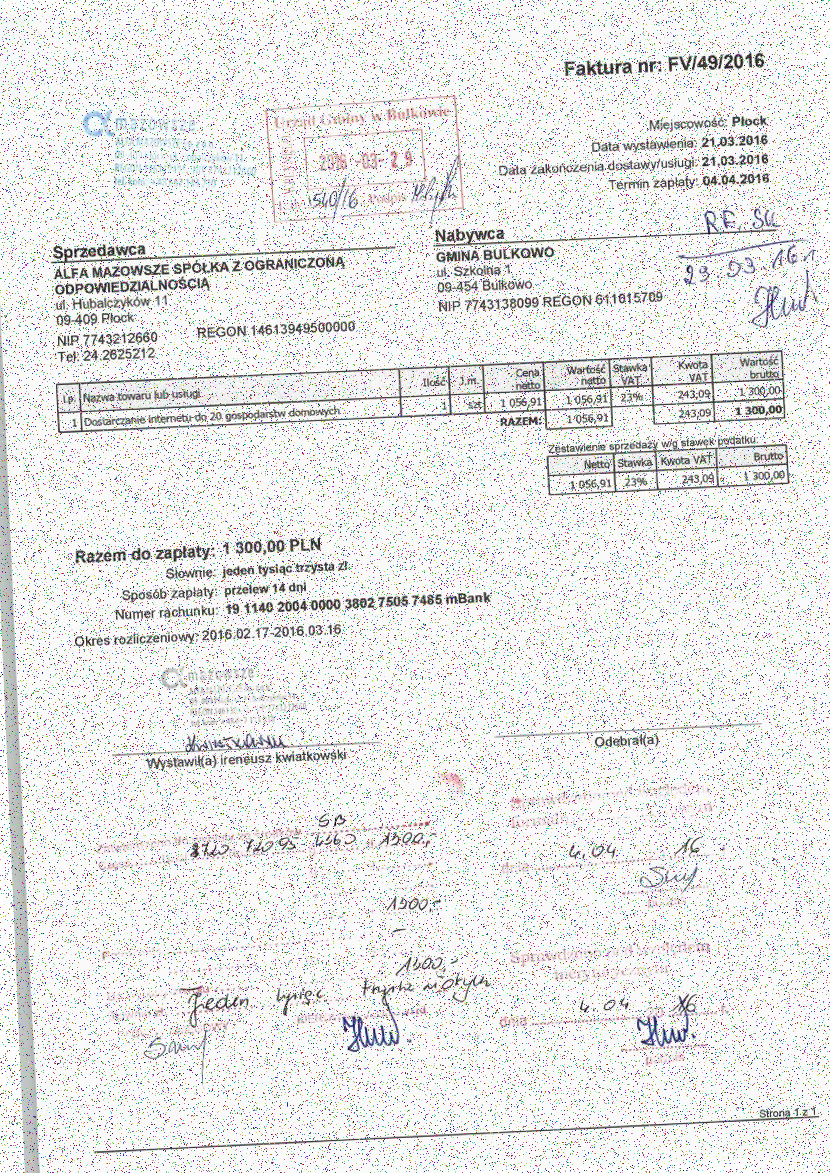
\includegraphics[width=.33\linewidth]{testing/ALFA-sap.jpg}
  \end{subfigure} \par\medskip
  \begin{subfigure}{\linewidth}
  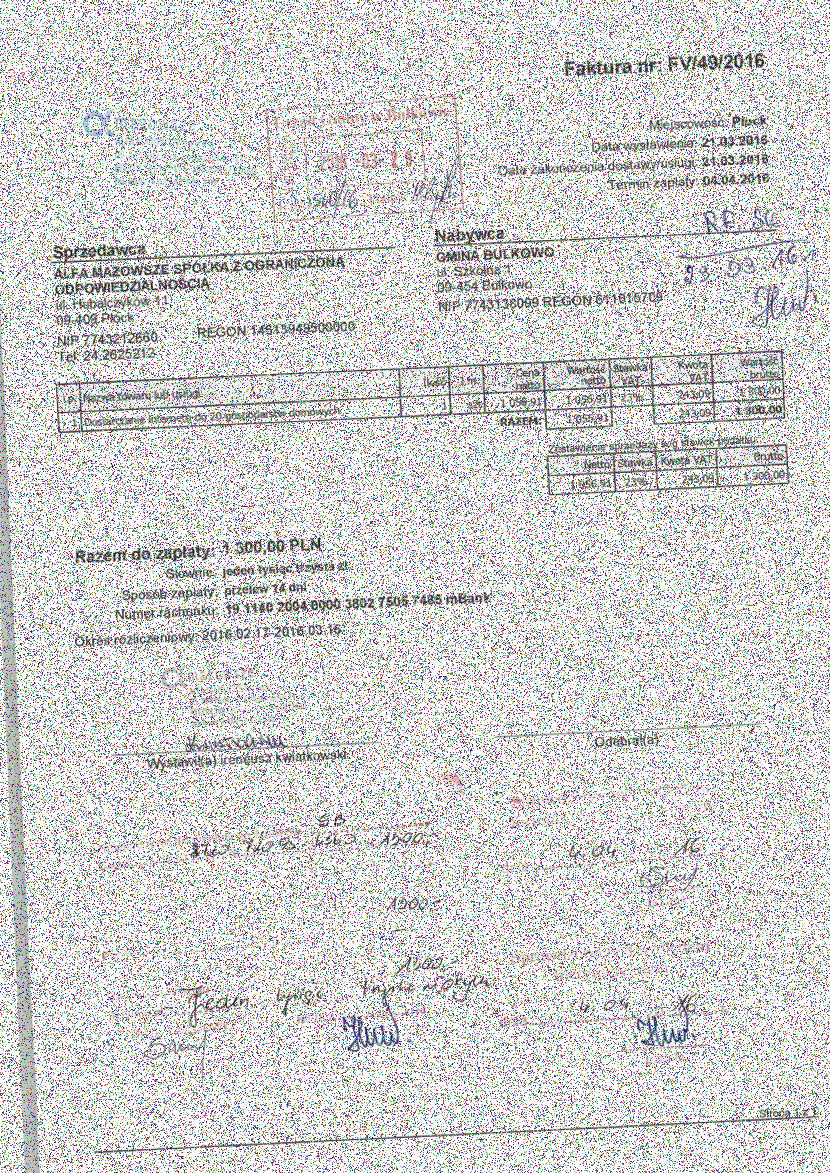
\includegraphics[width=.33\linewidth]{testing/ALFA-sap25.jpg}
  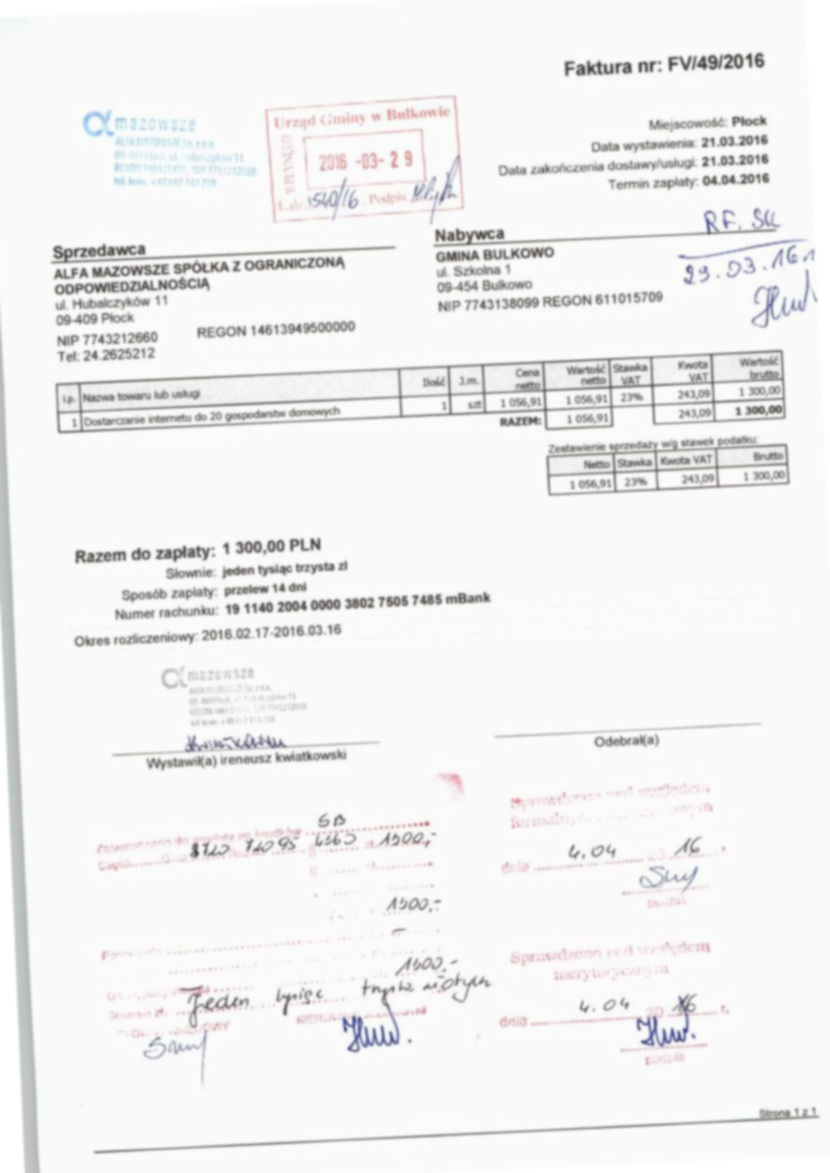
\includegraphics[width=.33\linewidth]{testing/ALFA-gauss.jpg}\hfill
  \end{subfigure}
  \caption{Obrazy testowe} \label{fig:testowe}
\end{figure}


\subsection{Obrazy testowe}

Oba programy zostały przetestowane na pięciu obrazach testowych. Obrazy 1 i 2 to prawdziwe skany faktur, wykonane w zadowalającej jakości \footnote{Skany zostały udostępnione przez urzędy gmin Bulkowo i Otmuchów jako informacja publiczna. Na mocy ustawy z dnia 6 września 2001 r. o dostępie do informacji publicznej, obrazy takie mogą być swobodnie przetwarzane i rozpowszechniane.}, natomiast obrazy 3, 4 i 5 są to obrazy z arbitralnie nałożnym szumem:
\begin{itemize}
\item W obrazie 3 wartości 10\% pikseli (wybranych losowo) zostały zamienione na losowe.
\item W obrazie 4 podobnie jw., tyle że zmodyfikowane zostało 25\% pikseli.
\item W obrazie 5 zostało zastosowane rozmycie Gaussa.
\end{itemize}

\begin{figure}
  \begin{subfigure}{\linewidth}
  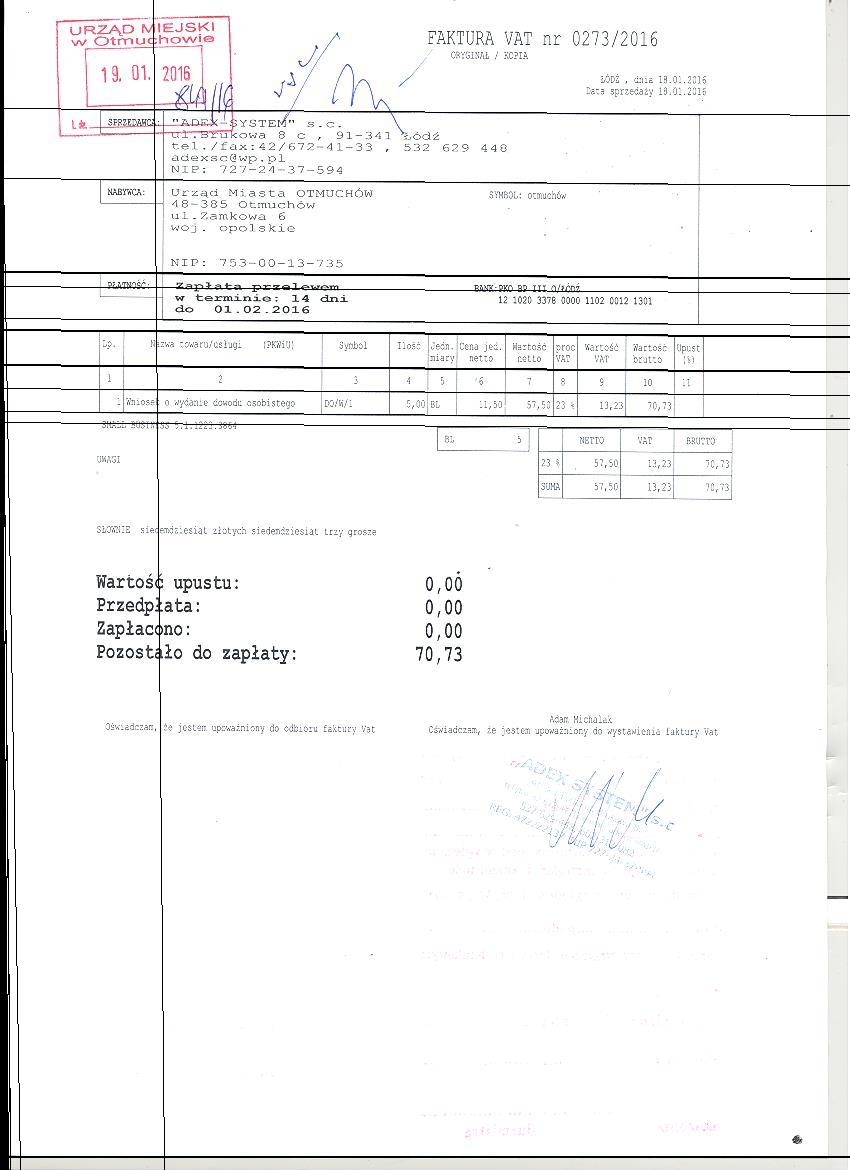
\includegraphics[width=.33\linewidth]{own/ADEX.jpg}\hfill
  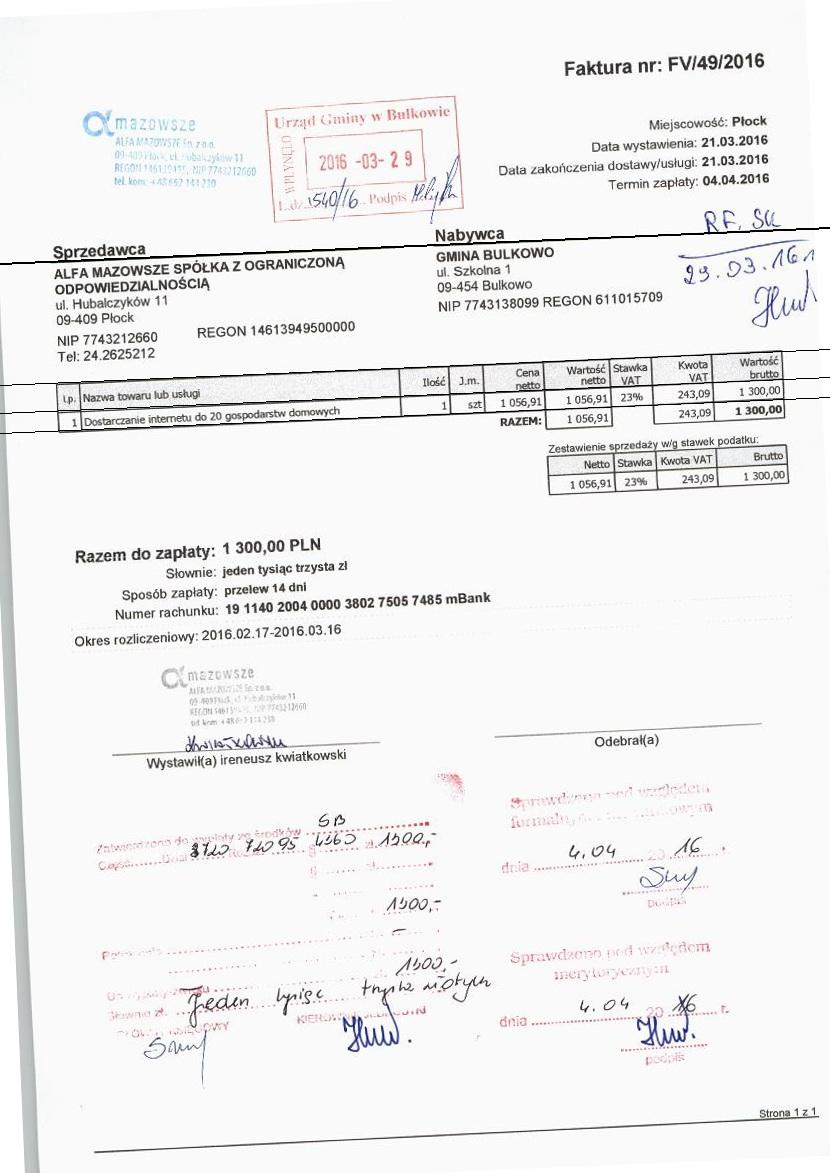
\includegraphics[width=.33\linewidth]{own/ALFA.jpg}\hfill
  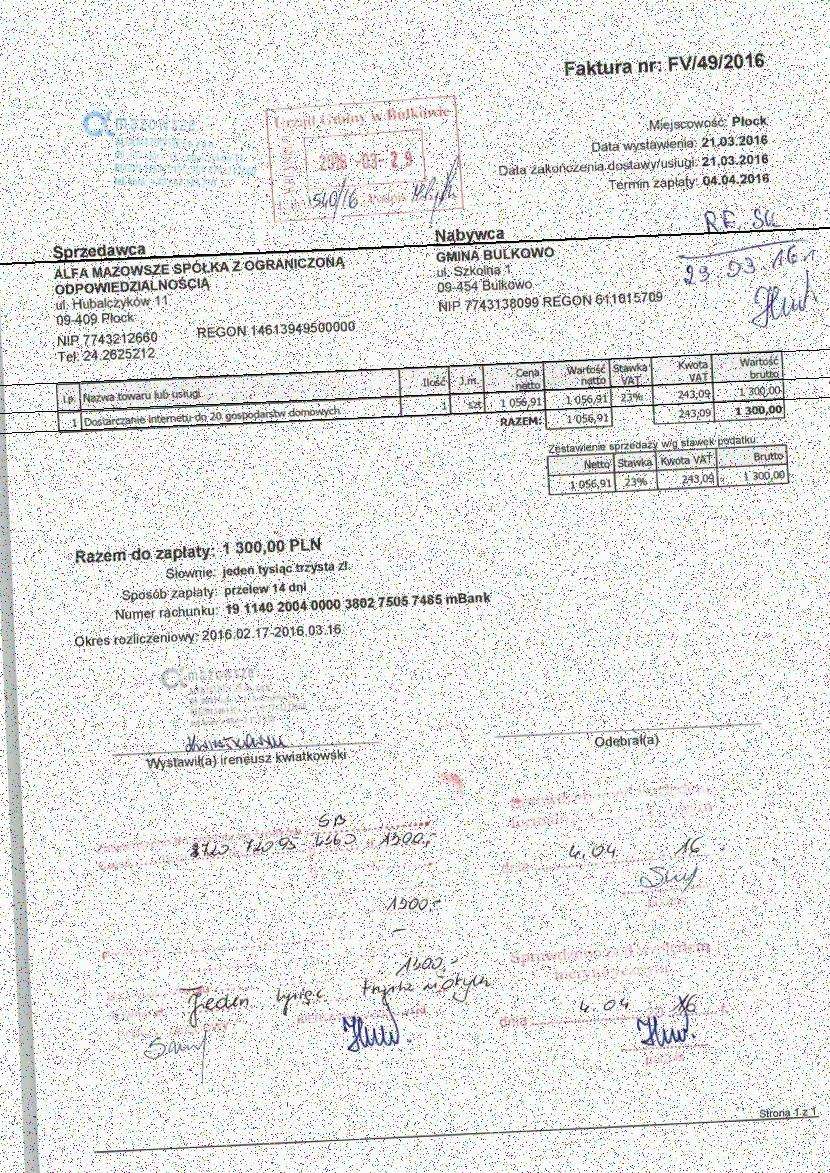
\includegraphics[width=.33\linewidth]{own/ALFA-sap.jpg}
  \end{subfigure} \par\medskip
  \begin{subfigure}{\linewidth}
  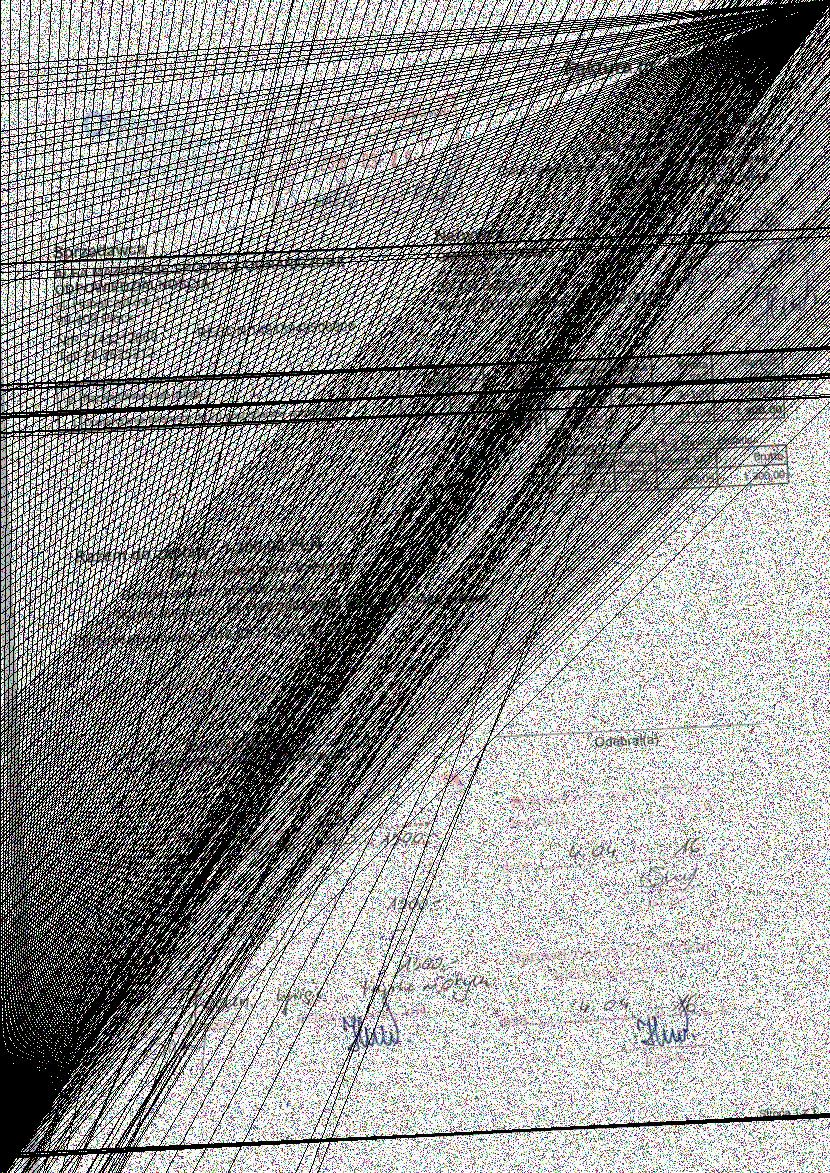
\includegraphics[width=.33\linewidth]{own/ALFA-sap25.jpg}
  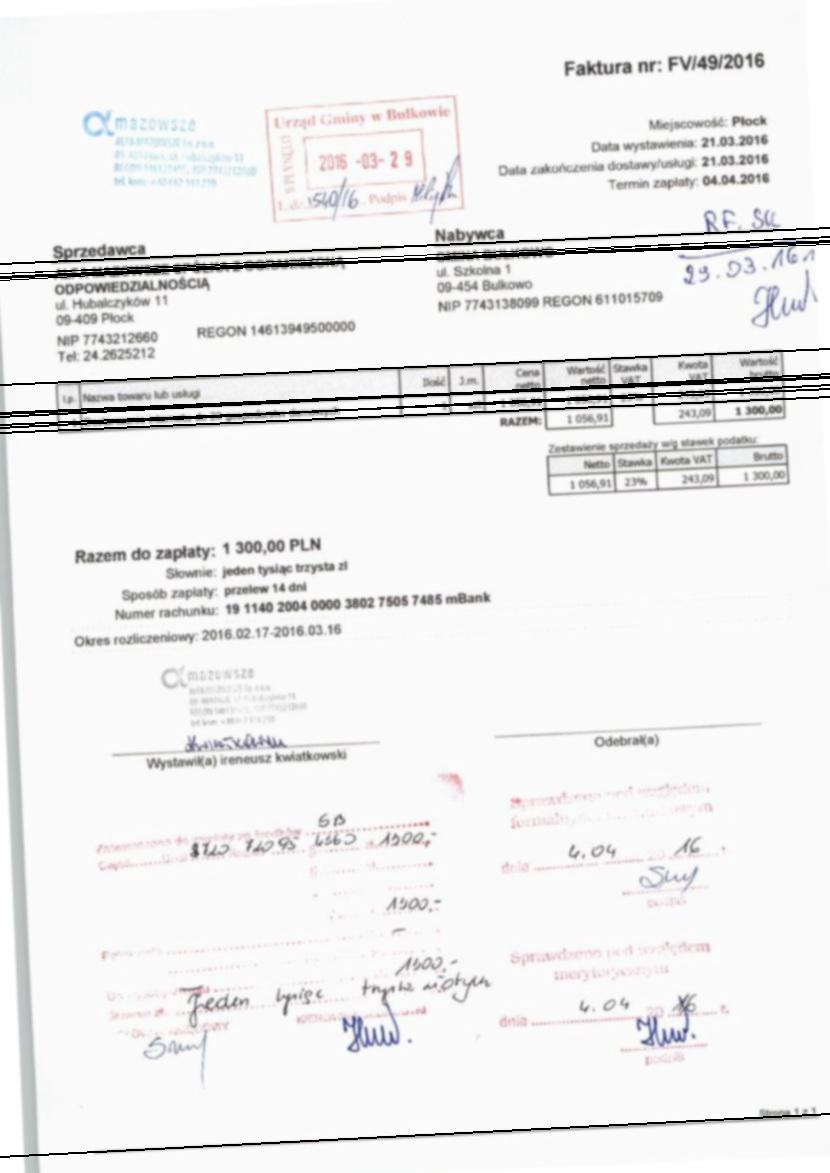
\includegraphics[width=.33\linewidth]{own/ALFA-gauss.jpg}\hfill
  \end{subfigure}
  \caption{Obrazy testowe z nałożonymi liniami wykrytymi przez własną implementację} \label{fig:java}
\end{figure}


Wszystkie te dokumenty zawierają tabelki (z produktami i z podsumowaniem stawek VAT), które należy wykryć. Idealnie, algorytm powinien wykryć tylko linie tworzące tabele, co pozwoliłoby wykryć położenie samej tabeli przez zlokalizowanie obszaru przecięcia linii.

Miniaturki obrazów są widoczne na ilustracji \ref{fig:testowe}, zaś pełne wersje znajdują się w \href{https://github.com/ciekawylogin/hough}{repozytorium} w katalogu \texttt{docs/testing}.


\begin{figure}
  \begin{subfigure}{\linewidth}
  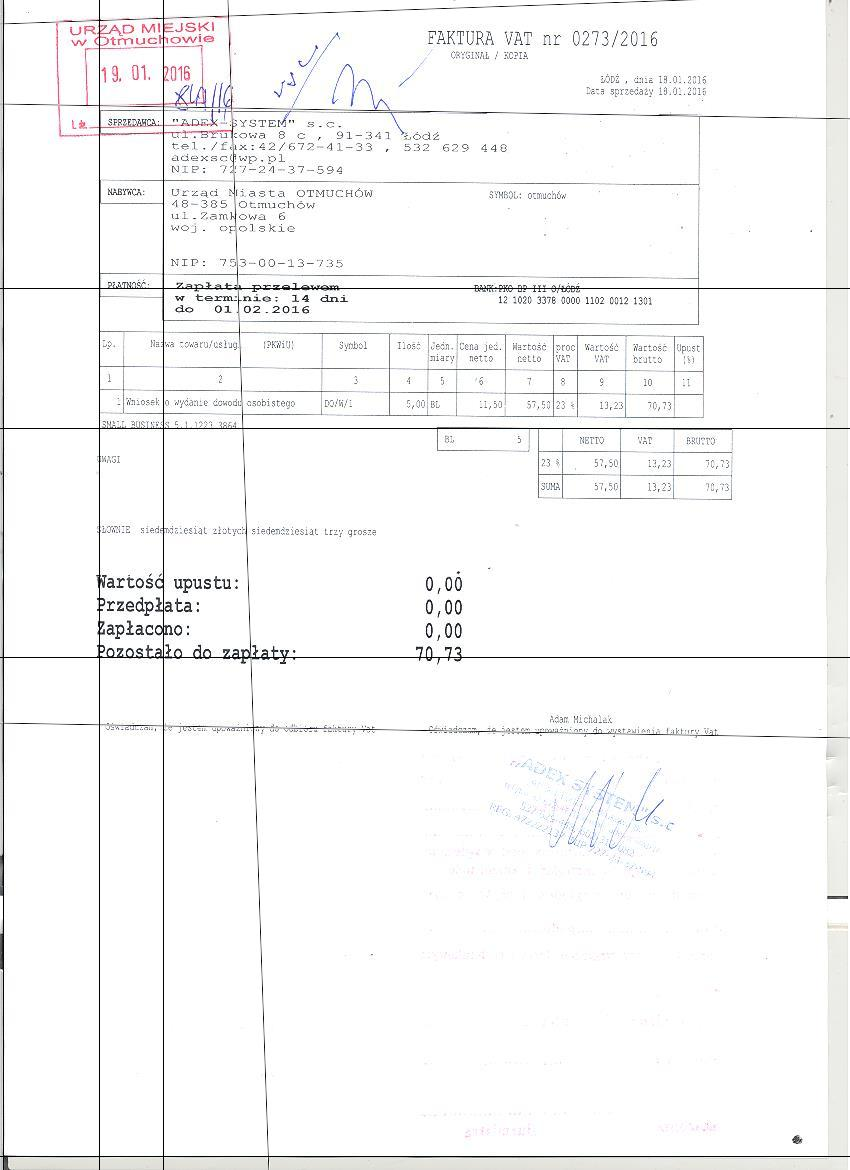
\includegraphics[width=.33\linewidth]{im/ADEX.jpg}\hfill
  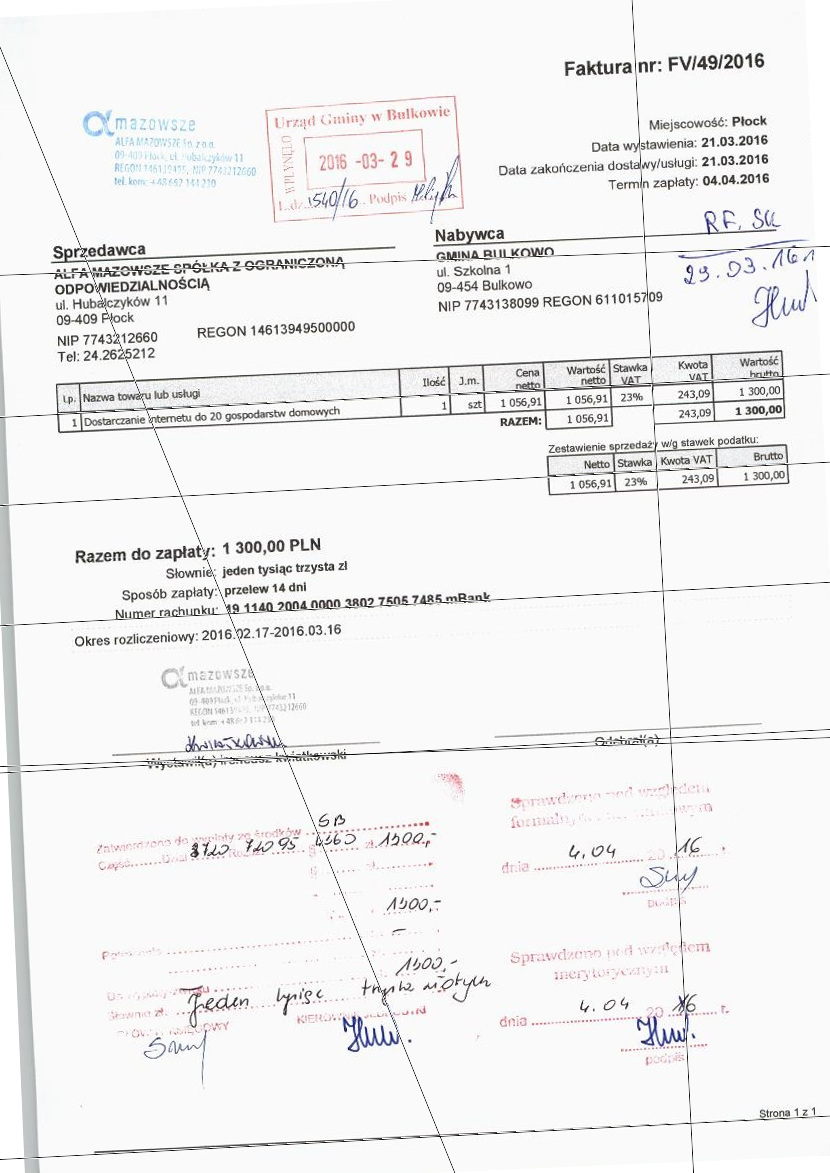
\includegraphics[width=.33\linewidth]{im/ALFA.jpg}\hfill
  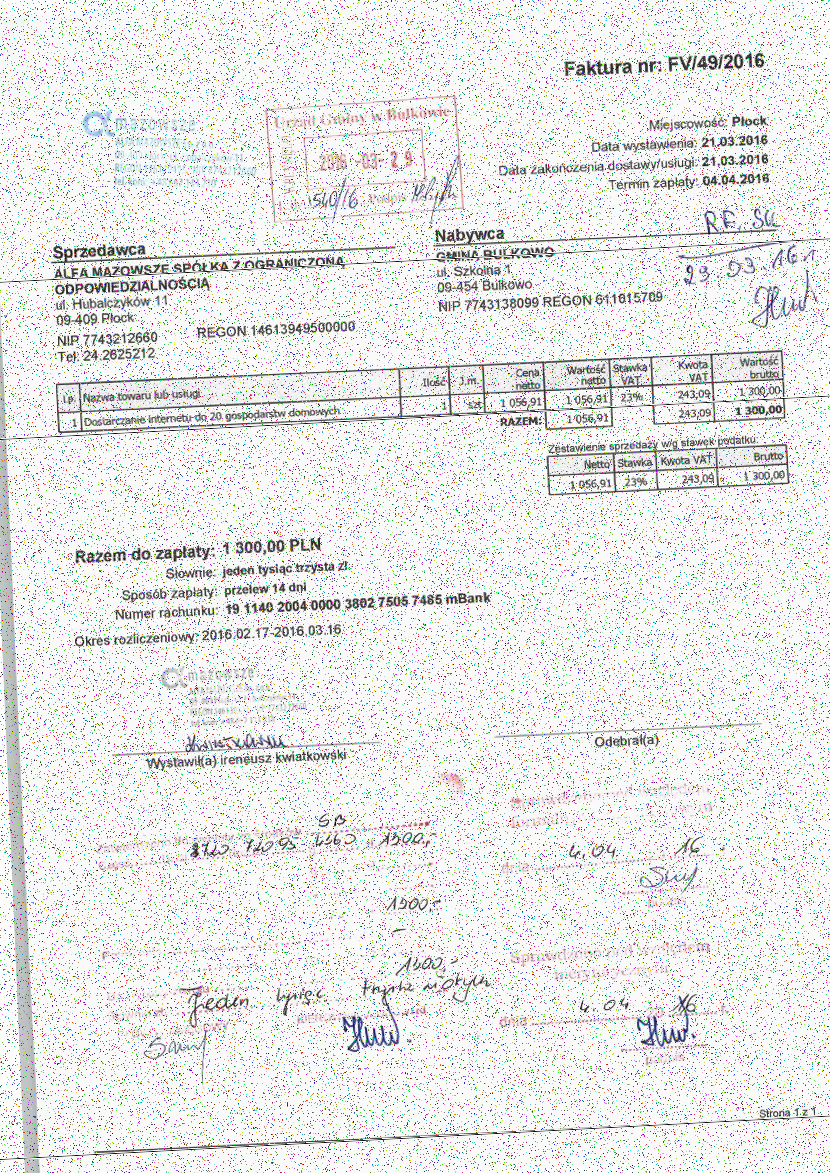
\includegraphics[width=.33\linewidth]{im/ALFA-sap.jpg}
  \end{subfigure} \par\medskip
  \begin{subfigure}{\linewidth}
  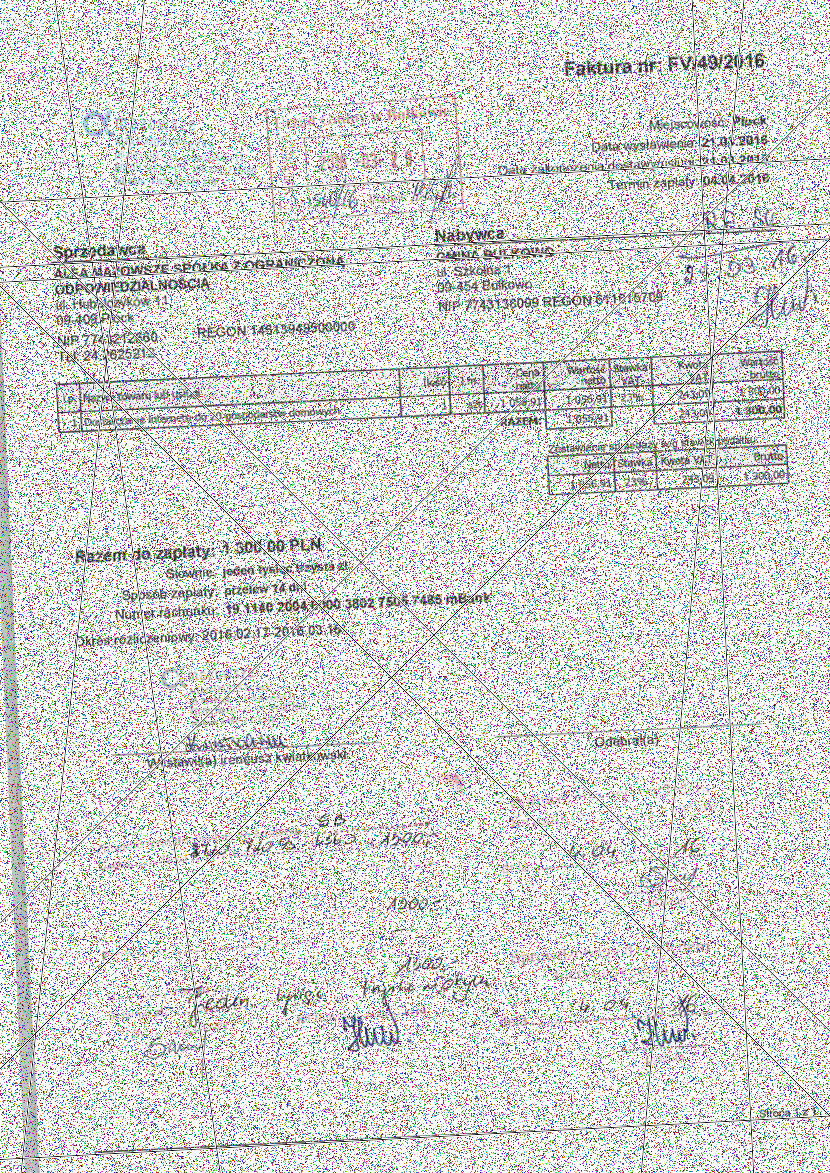
\includegraphics[width=.33\linewidth]{im/ALFA-sap25.jpg}
  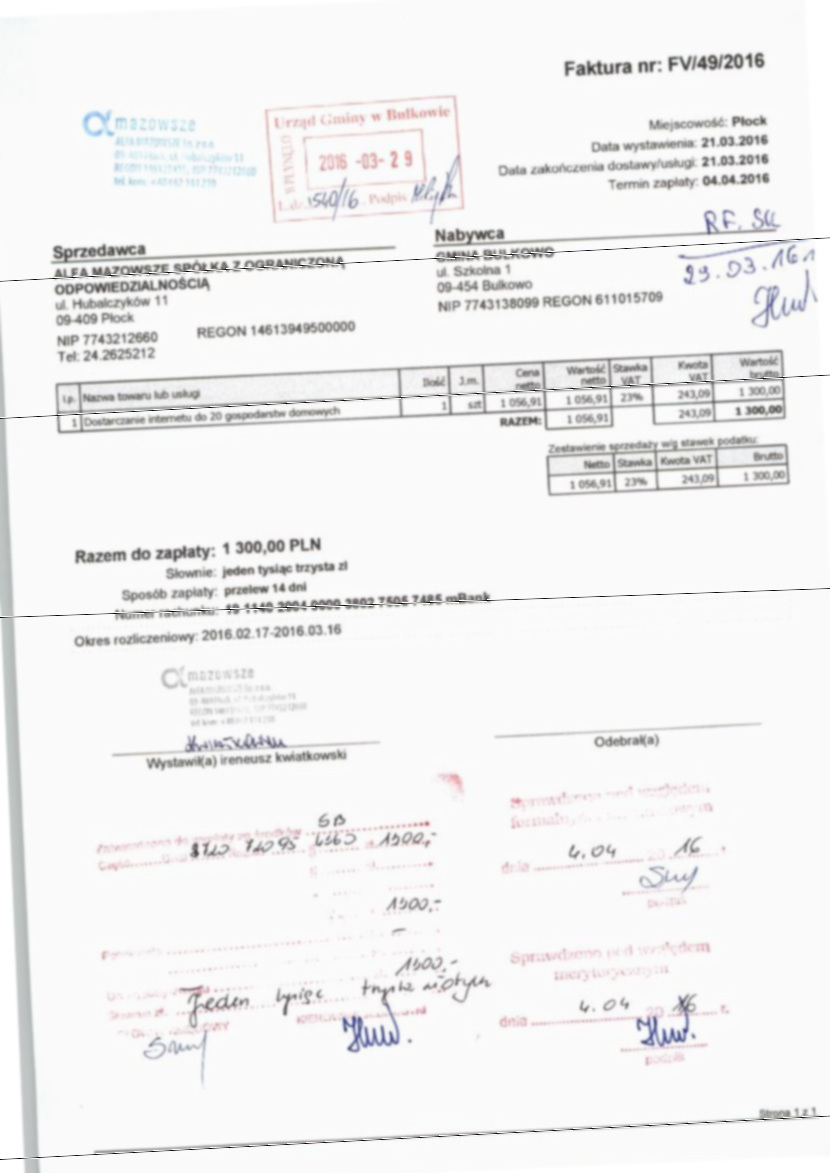
\includegraphics[width=.33\linewidth]{im/ALFA-gauss.jpg}\hfill
  \end{subfigure}
  \caption{Obrazy testowe z nałożonymi liniami wykrytymi przez \texttt{Imagemagick}} \label{fig:im}
\end{figure}


\subsection{Wyniki}
Wyniki działania zaimplementowanego programu zostały pokazane na ilustracji \ref{fig:java}. Dla porównania, wyniki działania \texttt{Imagemagick} przedstawia ilustracja \ref{fig:im}. Pełne wersje obrazów zostały zamieszczone w repozytorium, odpowiednio w katalogach \texttt{docs/own} i \texttt{docs/im}.

W obu przypadkach, linie zostały nałożone na oryginalne obrazy. 

\subsection{Omówienie wyników}
\begin{enumerate}
\item Obraz 1 jest ,,najłatwiejszym'' z obrazów tesotwych, nie powinno zatem dziwić, że oba programy znalazły poziome linie tworzące tabele. \texttt{Imagemagick} znalazł również jedną z linii pionowych. Jednak zwrócone zostały nie tylko one - w obu przypadkach część zdetekowanych linii to po prostu linia bazowa tekstu.
\item Obraz 2 --- podobnie jak w poprzednim przypadku, obie implementacje znalazły większość poziomych linii tworzących tabele, a \texttt{Imagemagick} także jedną z linii pionowych. Oba detektory znalazły też poziomą linię oddzielającą napisy ,,sprzedawca'' i ,,nabywca'' od sekcji danych sprzedawcy i nabywcy. \texttt{Imagemagick} ,,znalazł'' też skośną linię, której nie widać gołym okiem -- jest to zbiór krótkich, skośnych linii, będących w większości fragmentami liter (np. ,,y'', ,,W''), które okazują się być współliniowe.
\item Obraz 3 to obraz zaszumiony. Tu w przypadku mojej implementacji nie widać różnicy w stosunku do obrazu 2, zaś w przypadku programu \texttt{Imagemagick} zostało wykrytych znacznie mniej linii -- wynika to z faktu, że algorytm Otsu zwrócił inną wartość progu binaryzacji na skutek istnienia szumu.
\item Obraz 4 jest zaszumiony tą samą metodą co poprzedni, jednak w dużo większym stopniu. Na tym obrazie własna implementacja zaczęła wyraźnie ,,gubić się'' i znajdować wiele nieistniejących linii. Linie te w większości są po prostu zbiorami punktów szumu, które przypadkowo akurat okazały się współliniowe. \texttt{Imagemagick} poradził sobie nieporównywalnie lepiej -- ,,znalazł'' co prawda kilka nieistniejących linii, ale było ich znacznie mniej.
\item Obraz 5, rozmyty za pomocą rozmycia Gaussa, w przypadku własnej implementacji spowodował ,,rozszczepienie'' znalezionych prostych. Ponadto, więcej linijek tekstu zostało uznanych za linie. W przypadku  \texttt{Imagemagicka} wpływ rozmycia był wyraźnie mniejszy.
\end{enumerate}

\section{Wnioski}
\begin{itemize}
\item Zaimplementowany przeze mnie algorytm w przypadku niezaszumionych i słabo zaszumionych obrazów ma skuteczność podobną do gotowego rozwiązania. 
\item W przypadku obrazów zaszumionych (4 i 5), \texttt{Imagemagick} poradził sobie zdecydowanie lepiej, choć również popełniał błędy. 
\item Na żadnym z obrazów testowych żadne z rozwiązań nie wykryło obramowań tabeli z pełną skutecznością. Wynika to z faktu, że linie tekstu są w przestrzeni Hougha na tyle ,,podobne'' do prostych, że algorytm zwyczajnie nie jest w stanie ich rozróżnić. Można próbować dostosować wartość progowania $p$, jednak ustawienie jej na zbyt wysoką wartość powoduje, że linie tworzące obamowanie tabeli w większości nie zostaną wykryte, a zbyt niską -- że większość tekstu zostanie uznana za linie. Sugeruje to, że wykrywanie obramowań tabeli na tego typu dokumentach wymaga zastosowania algorytmu bardziej zaawansowanego niż algorytm Hougha.
\end{itemize}

\begin{thebibliography}{9}

\bibitem{imagemagick}
  \textit{Use ImageMagick® to create, edit, compose, or convert bitmap images},
   \href{https://www.imagemagick.org/script/index.php}{https://www.imagemagick.org/script/index.php}

\bibitem{hough}
  Hough, Paul\\
  \textit{Method and means for recognizing complex patterns}, 
  \href{https://www.google.com/patents/US3069654}{https://www.google.com/patents/US3069654}
  
\bibitem{duda}
  Duda, R. O., Hart P. E.\\
  \textit{Use of the Hough Transformation to Detect Lines and Curves in Pictures},  \\
  Communications of the ACM, nr 15, str. 11–15 (styczeń 1972)
 
\end{thebibliography}



\end{document}